% http://www.idsc.ethz.ch/education/theses-semester-projects.html
% IDSC LaTeX Thesis Template
% 
% Author(s):	Eric Müller
% 				Institute for Dynamic Systems and Control
% 				Swiss Federal Institute of Technology (ETH) Zurich
% 
% Created:		2004/04/02  (Eric Mueller)
% 
% Notes: Has been tested on Windows 7 + MikTeX + TeXnicCenter
%
% Revisions: 	2009/05/29  (Soren Ebbesen)
% 				    2011/03/22	(Soren Ebbesen)
%             2013/03/08	(Soren Ebbesen)
%             2014/03/13	(Soren Ebbesen)
% ______________________________________________________________________________
% \documentclass[10pt,twoside,a4paper,fleqn]{report}
\documentclass[10pt,twoside,a4paper,fleqn]{scrbook}

%custom commands for comments of Supervisor (sv), phd candidate(pc)
\newcommand{\sv}[1]{\textcolor{red}{{\textbf{SV:}}~#1}}    
\newcommand{\pc}[1]{\textcolor{cyan}{{\textbf{PC:}}~#1}} 

% text color
\usepackage[svgnames,x11names,table]{xcolor}

\usepackage[english,mt]{ethidsc} % Special IDSC styles and commands      	
								 % {german}/english: language of headings, etc.
								 % {st}/bt/mt: {semester}/bachelor/master thesis
\usepackage{caption, subcaption}
% Image position [H]
\usepackage{float} % table position
%\usepackage{csvsimple} %(if want to add tables from csv. Otherwise use: https://www.tablesgenerator.com/latex_tables and import them from File->import csv file...)
% Tables with cells that take multiple rows
\usepackage{multirow}
% Allow for a new line in the same cell of a table (https://tex.stackexchange.com/questions/2441/how-to-add-a-forced-line-break-inside-a-table-cell/19678)
\usepackage{makecell}
% forests (used to represent classes in the code)
\usepackage[edges]{forest}
% forests (attempt II)
\usepackage{forest}
% acronym
\usepackage{acronym}
% to include a pdf with the title page
\usepackage{pdfpages}

\hypersetup{ 	
pdfsubject = {Thesis},
pdftitle = {},
pdfauthor = {},
colorlinks=true,
urlcolor=DarkBlue,
linkcolor=DarkBlue,
citecolor=DarkBlue,
filecolor=DarkBlue,
pdfborder={0 0 0}
}


\usetikzlibrary{arrows.meta}
\forestset{
  dir tree/.style={
    for tree={
      parent anchor=south west,
      child anchor=west,
      anchor=mid west,
      inner ysep=1pt,
      grow'=0,
      align=left,
      edge path={
        \noexpand\path [draw, \forestoption{edge}] (!u.parent anchor) ++(1em,0) |- (.child anchor)\forestoption{edge label};
      },
      font=\sffamily,
      if n children=0{}{
        delay={
          prepend={[,phantom, calign with current]}
        }
      },
      fit=band,
      before computing xy={
        l=2em
      }
    },
  }
}
% accents and special characters
%\usepackage[utf8]{inputenc}

% Page header (don't change)________________________________________________
\setlength{\parindent}{0em}                 % Disable parindent
\rhead[\nouppercase{\rightmark}]{\thepage}  % Special headings
\lhead[\thepage]{\nouppercase{\leftmark}}   % Special headings
\cfoot{}                                    % Special headings


% Title page (please fill in)____________________________________________
\title{Thesis title here}


\studentA{PhD Candidate Name}
\ethidA{}
\semesterA{}
\emailA{}


\supervision{Prof. Dr. Supervisor}
\date{Month YEAR}
%\type{Ph.D. Thesis}
%\identification{IDSC-XX-YY-ZZ} 		% Project identifier

\infopage
%\declaration


% Begin document___________________________________________________________
\begin{document}
\maketitle 							% Create title page


\newlength{\originalVOffset}
 \newlength{\originalHOffset}
 \setlength{\originalVOffset}{\voffset}   
 \setlength{\originalHOffset}{\hoffset}
 \setlength{\voffset}{0cm}
 \setlength{\hoffset}{0cm}
 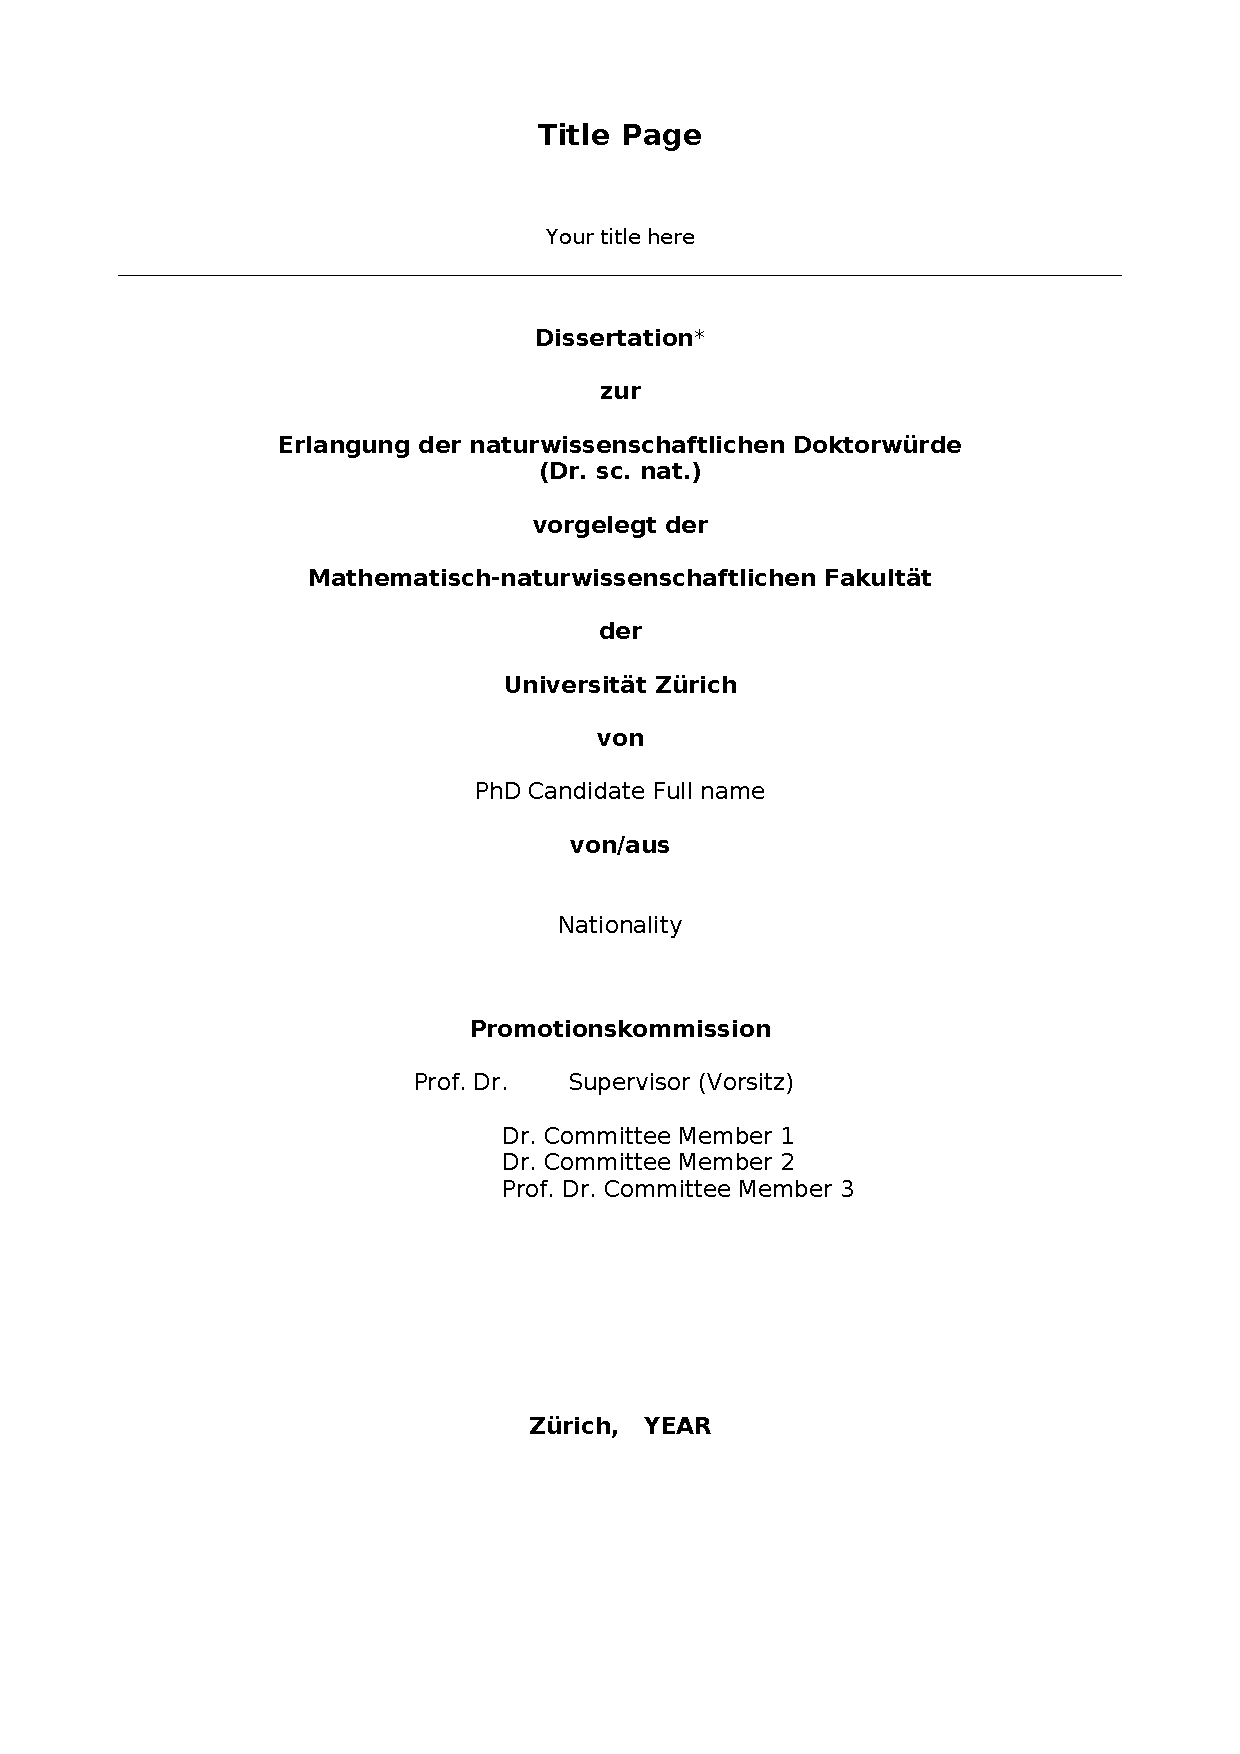
\includepdf[pages=-]{Titelblatt.pdf}
 \setlength{\voffset}{\originalVOffset}
 \setlength{\hoffset}{\originalHOffset}
 
% Preamble_______________________________________________________________

\pagenumbering{roman} 				% Begin roman page numbering (i,ii,...)

%---------------------------------------------------------------------------
% Preface

\chapter*{Abstract}
 \addcontentsline{toc}{chapter}{Abstract}

 \newpage
 
 \chapter*{Acknowledgements}
 \addcontentsline{toc}{chapter}{Acknowledgements}
 

 \newpage

%---------------------------------------------------------------------------
% Table of contents

 \setcounter{tocdepth}{2}
 \tableofcontents

 \newpage

%---------------------------------------------------------------------------
% Symbols

\chapter*{Nomenclature}\label{chap:symbole}
 \addcontentsline{toc}{chapter}{Nomenclature}

\section*{Symbols}


\section*{Acronyms and Abbreviations}
\input{biblio/acronyms_list}


 \newpage

%---------------------------------------------------------------------------


\pagestyle{fancy}               	% Fancy headings
\pagenumbering{arabic}				% Begin arabic page numbering (1,2,...)



% Chapters______________________________________________________________________


\chapter{Introduction}
\label{chapter:introduction}
\section{Section}
\subsubsection{subSection}
%\subsection{Thesis Objectives}
\section{Thesis Outline} %include objectives here

Add a sentence with a random citation~\cite{AER-Caltech-Memo}.
\newpage
	

% Appendix______________________________________________________________________
\appendix
 \chapter{Appendix Title}
 \label{appendix:app-title}
 

\chapter{Supplementary Material}
\label{appendix:supplementarymaterial}




% Bibliography__________________________________________________________________
% Literature (Additional references can be added to the .bib-file manually, or by using, for example, the free application JabRef). Compile in the following order: latex -bibtex -latex -latex

\bibliographystyle{plain}
\bibliography{biblio/biblioncs}

\end{document}
